\documentclass[french]{article}
\usepackage[utf8]{inputenc}
\usepackage{graphicx}
\usepackage{french}

\usepackage{natbib}
\usepackage{xcolor}
\usepackage{listings}
\usepackage{fancyhdr}
\usepackage{verbatim}
\usepackage{hyperref}
\usepackage[T1]{fontenc}
\usepackage{placeins}
\usepackage{amssymb}
\usepackage{float}
\usepackage{caption}
\usepackage{subcaption}
\usepackage{dirtytalk}

\title{ \Huge \textbf{Open Mapping}}
\author{ BHATI Vikram - BOUZIDI Imane \\ ISSAOUI Ali - LEBDAOUI SELMANE \\ 
     \\ Encadré par: \\ \\ S. ARCHIPOFF \\ D. RENAULT}
\date{Avril 2019}

\begin{document}

\maketitle
\begin{center}

\includegraphics[scale=0.40]{enseirb.png}
\end{center}

\newpage

\tableofcontents

\newpage

\section{Introduction}
\subsection{Présentation du sujet} %% Imane


Dans ce projet intitulé Open Mapping Service, nous étions amenés à manipuler les graphes afin d’exploiter des données cartographiques. Dans un premier temps, notre tâche consistait à construire un graphe à partir des données au format XML ( fournis par ... ) , dans un second temps, il s’agissait d’implémenter un ensemble d’algorithmes afin d’exploiter ces graphes : calculer les distances entre des noeuds, extraire des itinéraires et des cycles, etc… Finalement, nous avons implémenter un serveur HTTP pour afficher les résultats en utilisant le conteneur SVG. Ce rapport a pour but de décrire le déroulement du projet. \newline

Dans un premier temps, nous allons présenter comment nous avons géré le projet. Nous avons choisi de répartir les tâches entre les différents membres du groupe. Cette première partie serait également l’occasion pour nous de justifier notre choix de certaines structures et du Hash table que nous avions jugés aptes à répondre aux consignes du sujet et adaptés à nos besoins. \newline

Dans un second temps nous présenterons, d’une manière spécifique, les différentes parties du projet telles que nous les avons imaginées et conçues. Nous décrirons le fonctionnement de chaque algorithme implémenté. Nous saisirons l’aubaine, dans cette meme optique « technique », pour faire part de nos impressions sur le projet et les difficultés techniques rencontrées ainsi que les voies de recherches ouvertes.\newline

Comme dans tout projet de programmation, il était nécessaire que nous nous assurions que notre code fonctionne bien et répond aux exigences du sujet, sans erreur, et produit ce pour quoi il a été construit. Pour cette raison, nous avons conçus des tests dont la principale fonction était de mettre sous la loupe chaque travail fait et de s’assurer que ce dernier répond aux consignes.\newline

Enfin, la dernière partie serait consacrée à mettre en exergue les perspectives ouvertes, ce que nous n’avons pas pu faire, les limites des solutions que nous avons proposées.\newline

Nous espérons que vous prendrez autant de plaisir à lire ce rapport que nous en avons pris durant le déroulement de ce projet. 

\newpage
\section{Organisation du projet}
\subsection{Gestion du travail et répartition des taches} %% Imane
Pour un bon déroulement du projet, il était nécessaire que nous déterminions les différentes tâches et les répartir entre nous. Pour cela, et après avoir pris connaissance du sujet, nous avons défini les solutions aptes à répondre aux consignes pour, finalement, déterminé les tâches à accomplir. \newline 
Les deux principaux enjeux que nous avons cernés pour ce projet sont: 

\begin{enumerate}
\item Manipuler les données au format XML .  
\item Convertir ces données en des graphes exploitables.
\end{enumerate} 
Les principales tâches qui ont aiguillé notre projet sont les suivantes : \newline

\begin{itemize}
\item Chargement des fichiers au format osm et leur transcription en un format de graphe adéquat.
\item Choix des structures du graphe et des sommets
\item Pondération du graphe
\item Exploitation du graphe (1) : calcul d’un itinéraire entre deux sommets, extraction du plus court chemin 
\item Exploitation du graphe (2) : calcul du cycle de longueur minimale (problème du voyageur de commerce) 
\item Affichage des maps dans un serveur HTTP à l'aide du conteneur SVG.
\end{itemize}


Nous avons travaillé en autonomie sur ses tâches en partageant les solutions utilisées et expliquant clairement chaque modification effectuée. Ainsi, chaque vendredi après-midi a été l’occasion pour nous de mettre le point sur nos avancements et tenir compte Mr ARCHIPOFF de notre travail.  

\subsection{Le choix des structures} 

Pour représenter les sommets, on a choisi la structure \textbf{\#vertex} où on a l'identifiant du sommet noté  \textit{id}, la latitude du sommet notée \textit{lat} , la longitude du sommet notée \textit{lon} et la liste des voisins notée \textit{way}
\begin{center}
                               $\{id_1:lon:lat:way\}$
\end{center}
Pour la représentation du graph , on a définit une structure \textbf{\#graph} qui contient une table de hachage qui à chaque clé : $id$ associe un \textbf{\#vertex} . L'id contenu dans ce vertex doit etre le même que l'id se trouvant dans la table de hachage, 
\begin{center} 
                   $(\{id_1:V_1\},\{id_2:V_2\},..., \{id_n:V_n\})$ avec $(vertex-id~V_n)=id_n$
\end{center}

\subsection{Le choix du Hash table}%% Vikram
Dans le projet, le choix de la structure de graph se prêtait naturellement à l'implémentation par liste d'adjacence. Toutefois, cela a un cout en temps assez élevé: au pire l'on accède à une donnée en $O(n)$ (n étant de nombre de noeuds du graphe), au mieux en $O(\log_2(n))$ (par dichotomie). Dans tous les cas, cette approche devient très handicapante pour un nombre important de noeuds. Et c'est exactement le cas pour les fichiers osm que l'on traite. C'est pourquoi, il nous a semblé plus judicieux d'utiliser une table de hachage dont l'accès et la mise à jour des noeuds se fait en $O(\log(N))$ (où N est une constante)
\footnote{lien vers la documentation Racket du Hash Table mentionnant la complexité: $https://docs.racket-lang.org/reference/hashtables.html$}.

\section{Explication des algorithmes et des implémentations choisies}
\subsection{Le graphe} 
La fonction \textit{{c}reate-vertex()} sert à créer à partir d'un identifiant \textit{id}, des coordonnées \textit{lat} et \textit{lon} et la liste des voisins \textit{way} un sommet. La fonction \textbf{add-vertex()} sert à ajouter un sommet à un graph. A noter que chaque sommet dans le graph dispose d'un id unique, et qu'il reste beaucoup de fonctions basiques de traitement du graphe spécifiques à chaque fichier source.
\subsection{Passage de l'Osm au graph} 
Cette partie explique le processus permettant de passer d'un fichier osm à un graphe. Tout d'abord, l'importation du fichier osm sous Racket conserve certaines normes de paranthésages qui nous ont semblé obsolètes pour les raisons suivantes: notre but étant d'extraire les noeuds sous forme de vecteur \textbf{(identifiant longitude lattitude liste:(voisin 1 voisin 2 ...))}, on a remarqué que les trois premières informations étaient toujours précédées du mot-clé \say{node} quand à la dernière information, elle était précédée de \say{way}. Ainsi, il suffisait d'abord d'effecteur un $flatten$ sur le fichier osm importé, suivi d'un $member$ pour trouver les mot-clés et ensuite récupérer les informations voulues.\newline

Dans notre implementation, on ne parcourt le fichier osm que 3 fois : la première pour $flatten$, la seconde pour créer la liste des noeuds avec les caractéristiques (identifiant longitude lattitude) et une troisième fois pour créer la liste des voisins comme liste de couple \textbf{(a b)} où a et b sont les identifiants des noeuds qui se suivent dans la section \say{way} du fichier osm. Bien que l'on aurait aimé regroupé ces deux derniers parcours (la liste des noeuds et la liste des voisins) en 1 seul, cela aurait impacté la simplicité et la lisibilité du code. 
\newline Enfin, l'étape finale consiste à croiser la liste des noeuds avec celle des voisins et à les insérer dans la table de hachage.\newline 

Une fois le graphe sous forme de table de hachage obtenu, il faut désormais le simplifier. Pour cela, on doit supprimer les noeuds de degrés exactement 2. En effet, si on considère trois noeuds \textbf{A, B} et \textbf{C}, tels que \textbf{B} est voisin avec uniquement \textbf{A} et \textbf{C} (\textbf{B} est alors de degré 2), et si l'on va de \textbf{A} vers \textbf{C}, alors il est inutil de spécifier que l'on passe par \textbf{B}. C'est la simplification qui a été choisie (imposée). \newline

Il y a deux façon de traiter le problème: \underline{la première} est de parcourir le graphe pour supprimer les noeuds dans une copie du graphe, et \underline{la seconde} consiste à supprimer directement dans le graphe au fur et à mesure. Nous avons choisi la seconde méthode par considération du coût en espace et en temps qu'impliquerait une copie d'un fichier osm imposant. De plus, peu importe la méthode choisie, le problème reste fondamentalement le même, ainsi, l'on pourrait toujours apporter des modification mineures pour passer d'une implémentation à une autre.
\label{osmgraph}
\subsection{Le serveur SVG}
\subsubsection{Manipulation basique}
Pour une manipulation basique du graphe, on utilise une première famille de fonctions qui générent une liste des données du graph telles que \textbf{keys()} qui retourne la liste de tous les identifiants et \textbf{list-lat()} qui génère la liste des latitudes. 
\newline
Le deuxième type de fonctions est celui pour lequel on extrait des sommets particuliers, par exemple, le sommet dont la latitude est maximale ou encore celui dont la latitude est minimale. A noter que dans l'entete du fichier donné OSM figurent les bornes inférieure et supérieure de la latitude et de la longitude, nous récupérons alors ces bornes à l'aide de la fonction \textbf{extremums()} .
\subsubsection{Manipulation avancée (1) - Représentation d'un graph}
On a d'abord songé à convertir les longitudes et les latitudes avant de procéder au dessin du graph pour une mise à l'échelle. On convertit par exemple la latitude \textit{lat} de la manière suivante: 
\newline
\begin{center}
    $coefficient\_lat * \frac{minlat-lat}{lat - maxlat}$
\end{center}

\begin{itemize}
    \item La fonction \textbf{circle-ray()} place un cercle (un point) pour un sommet. Pour placer tous les sommets d'un graph on utilise la fonction \textbf{graph-circles()} .  
    \item Pour relier deux vertex, on utilise \textbf{create-line()}. Pour relier tous les sommets d'un graph on utilise la fonction \textbf{graph-lines()}. 
    \item Pour insérer  du texte dans un point de coordonnées \{x;y\} on utilise la fonction \textbf{display-distance()}. 
    \item On trace l'itinéraire entre un vertex et ses voisins à l'aide de la fonction \textbf{vertex-lines()}. Les sommets et les aretes sont tracés avec \textbf{graph-map()}.
\end{itemize}

\subsubsection{Manipulation avancée (2) - Représentation d'un itinéraire}
Etant donné un itinéraire entre une liste de sommets.
\begin{enumerate}
\item La fonction \textbf{itinerary-circles()} place chaque sommet de l'itinéraire. 
\item La fonction \textbf{itinerary-lines()} trace les aretes entre chaque paire de sommets. 
\item \textbf{dijkstra-map()} sert à tracer le chemin le plus court entre deux sommets.

Enfin, la fonction \textbf{itinerary-map()} est la combinaison des deux fonctions précédentes c'est-à-dire elle place les sommets et les aretes à la fois.
\end{enumerate}
\subsubsection{Le serveur racket}
Dans le fichier \textit{server.rkt}, nous avons implémenté les différents fonctions qui servent à traiter les \textit{requests} du language Racket, afin de pouvoir récupérer l'url éxecutée. En effet, nous avons fait quatres \textbf{rules} comme il est précisé dans l'énoncé, $display, ~route, ~distance$ et $cycle$. La fonction \textit{server-dispatch} permet de récupérer l'url à exécuter et vérifie si le mot directement apr\`es $http://localhost:9000/$ et avant $\?$ correspond à l'un des \textit{définis} précedemment, si c'est le cas, elle appelle la fonction correspondante. 
\subsection{Parcours du graph et itinéraire}
Une première façon de chercher l'itinéraire entre deux noeuds est le parcours en profondeur. En effet, nous avons implémenté une fonction de parcours en profondeur, qui, étant donné un graphe et un noeud de départ parcourt la totalité des noeuds appartenant à la même composante connexe que le noeud de départ, suivant le trajet du parcours en pronfondeur. Commençant par une racine, on parcourt un premier fils puis tous ses fils récursivement, ensuite, on passe aux autres fils de la racine. Deux variables nous ont été utiles, une première variable nommée \textit{Marked} qui marque chaque élement par lequel on est déj\`a passé pour ne pas le parcourir une deuxième fois. Et la variable \textit{result} qui joue le rôle d'une pile enregistrant à chaque fois l'itinéraire entre la racine est le noeud en cours de traitement par la fonction. En effet, à chaque \textbf{appel récursif}, la liste empile le noeud en cours de traitement, mais une fois cet appel fini, la liste dépile ce noeud. De cette façon, dès que le noeud traité est celui qu'on recherche, la liste \textit{result} contient le trajet voulu à partir de la racine, et est donc retournée. Par contre, cette fonction a besoin d'un parcours en profondeur déj\`a effectué sur le noeud de départ pour décider si le noeud d'arrivé est joignable ou pas.

\subsection{La formule de Haversine} %% Imane
Puisque dans ce projet, nous recourons à la manipulation des graphes, il est évident que l'on ait besoin d'un outil de calcul des distances à partir des coordonnées des sommets. Conformément aux instructions de l'énoncé, nous avons utilisé la formule de Haversine :
\newline
\begin{center}
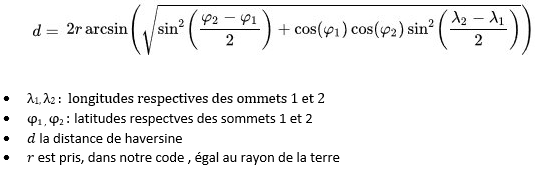
\includegraphics[scale=0.9]{hav.png}
\end{center}

Les résultats du calcul des distances avec cette formule ont été comparés aux valeurs données par l'outil qui nous a été livré en guise de ressource supplémentaire dans une page d'explication\footnote{lien vers la page d'explication livrant un outil de calcul de distance à partir de la latitude et de la longitude: $https://www.movable-type.co.uk/scripts/latlong.html$}. 

\subsection{Dijkstra}%% Imane

Dans cette partie, notre objectif était d'implémenter un algorithme permettant de trouver le plus court chemin entre deux sommets. Notre choix s'est naturellement porté sur l'algorithme de Dijkstra de par la simplicité de son principe mais aussi parce qu'il a été l'objet d'un enseignement dispensé dans le module Algorithmique des graphes.\newline 

Quoique le pseudo-code soit connu, l'implémentation de Dijkstra en fonctionnelle reste une tache ardue. Néanmoins, une façon facile de procéder consiste à décomposer le code en des fonctions auxiliaires qui interviendront toutes, à la fin, dans une boucle nommée \textbf{dijkstra\_loop()} dans notre code.\newline  

Le pseudo-code considéré est le suivant: \\
\begin{lstlisting}
      dijkstra(g,dis,sdep)                                  
      Initialisation(g,sdep)                                
      Q:= ensemble de tous les noeuds
      Tant que Q n'est pas un ensemble vide
      Faire
           s1:= min(Q)
           Q := Q privé de s1
           pour chaque noeud s2 voisin de s1 Faire
             maj_distances(s1,s2)
           fin pour
      fin tant que
\end{lstlisting}

Pour l'initialisation, la fonction \textbf{initial} prend en argument l'identifiant du sommet de départ, une liste des identifiants de tous les sommets du graph (y compris le sommet de départ) et une liste l \textit{(cette liste l serait toujours la liste vide au 1er appel)}. 
\newline
A l'issue de cette fonction, nous avons une liste de paires où chaque paire est sous la forme \textbf{(id\_sommet distance)} le champ distance est nul pour le sommet de départ et est égal à une valeur très grande (supérieure à toutes les distances considérées dans le problème) pour les autres sommets.\newline

\subsubsection{Une première version de Dijkstra}
Dans cette première version nommée \textbf{old-dijkstra} , nous avons choisi de manipuler surtout les identifiants des sommets et non pas la structure vertex (toute entière) puisque la structure du graph en Hash table nous permettait de récupérer, facilement, un vertex à partir de l'identifiant uniquement. Les deux enjeux principaux dans cette implémentation étaient de :

\begin{enumerate}

\item Avoir une structure qui nous permet de sauvegarder les sommets différents du sommet de départ et la distance séparant chacun de ces sommets du sommet de départ. Nous avons choisi d'utiliser une liste de paires, \underline{par exemple} : \textbf{((1 2.4) (2 3.01))} où le premier élément de la paire désigne l'identifiant du sommet et le deuxième représente la distance séparant ce sommet du sommet de départ (sdep) .

\item Mettre à jour à chaque itération cette liste de paires. La procedure majtabdis, prenant en argument une listedouble , une distance d et un sommet s met à jour la liste de telle sorte que la distance séparant le sommet de départ du sommet s devienne d.    
\end{enumerate}
La liste des paires est également la structure que nous avions privilégié pour sauvegarder les prédecesseurs/les voisins de chaque sommet. 

\subsubsection{La version fonctionnelle de Dijkstra}
Dans cette seconde version fonctionnelle nommée dijkstra, nous nous sommes basés une deuxième fois sur les tables de hachages, en effet, notre fonction \textit{initialize} génère à partir d'un graphe et un noeud de départ passés en paramètre une table de hachage dont l'élèment (id-v : (distance , predecessor)) o\`u distance est la distance séparant le vertex dont l'id est id-v du vertex de départ, cette distance étant inialisée à 10000, et predecessor représente l'identifiant du noeud prédecesseur du noeud d'id-v dans la liste de Dijkstra. Ensuite, on a eu besoin de la fonction \textit{find-min} prenant en paramètre \say{distance} qui est une table de hachage comme spécifié précedamment et Q qui est une liste de sommet. Cette fonction  retrouve le noeud le plus proche du noeud de départ. Puis, la fonction  \textit{maj\_distances} met à jour les distances stockées dans la table de hachage à chaque fois qu'elle trouve des noeuds plus proches. La fonction \textit{maj\_vertex} est une fonction intermediaire qui met à jours les distances de tous ses voisins. 
\newline 
Enfin, la fonction \textit{Dijkstra\_loop} représente la boucle du programme, elle prend en paramètres $g$ un graphe, $v$ un noeud de départ, $distances$ une table de hachage contenant les distances initiales et Q contenant la liste des ids des noeuds appartenant à la même composante connexe que le noeud de départ\footnote{fournie par un parcours en profondeur}. Dans la boucle principale, on cherche à chaque fois le noeud plus proche, mis à jour les distances de ses voisins et l'enlève de la liste Q.
Le résultat de ce traitement est une table de hachage contenant les ids des noeuds accessibles à partir du noeud de départ, Ensuite, pour trouver l'itinéraire il suffit de remonter les prédécesseurs du noeuds recherché dans la liste des distances jusqu'à ce qu'on trouve le noeuds de départ. Le résultat étant une liste d'élements ($id_{n}$, $distance_{n}$) avec distance étant la distance cummulée du noeud d'id $id_{n}]$ au noeud de départ. 

\subsection{Voyageur de commerce} %% Vikram
Le problème du voyageur de commerce est un problème classique d'optimisation, qui se résout efficamement à l'aide d'heuristiques comme celles des algorithmes génétiques ou des algorithmes de colonies de fourmis. Mais ces algorithmes sont plus adaptés à une implémentation itérative que fonctionelle.
\newline

Le but véritable de cette partie était de se familiariser au parcours de graphe en implémentant plusieurs stratégies de résolution du TSP (problème du voyageur de commerce). À commencer par la méthode des plus proches voisins, qui est une méthode na\"\i ve qui part d'un noeud arbitraire et construit un cycle en passant à chaque fois par le noeud le plus proche. La suivante est l'insertion minimale que l'on apellera greedy: on commence par une liste L de deux noeuds, et on ajoute les noeuds restants à L aux position où la distance est minimale. Une autre façon (peu commune) de résoudre le problème est de parcourir aléatoirement les sommets. \newline

\newpage
\section{Complexité des algorithmes, temps d'éxecution et mémoire}
\subsection{Le passage de l'Osm au graph et la réduction des sommets de degré 2}
Pour obtenir le graph, on doit passer par une série d'opérations sur le fichier osm: il faut d'abord le charger en mémoire, puis appliquer la procédure $flatten$. En notant K la longueur du fichier obtenu après avoir $flatten$ le fichier osm, obtenir le graph se fait en temps $O(K)$. En effet, on parcourt le fichier 3 fois au total: la première pour le flatten, la seconde pour obtenir la liste des sommets, et une troisème pour obtenir la liste des chemins (l'opération de stockage se faisant dans un hash table en $O(1)$).\newline
Notons g le graph obtenu. L'opération de réduction supprime un noeud de degré deux, notons le \textbf{A} dans la liste de ses voisins de \textbf{B} et \textbf{C} ce qui est au pire, en temps $O(\vert S\vert)$ (dans le cas où B ou C est voisin avec tous les sommets dans $S$). Ensuite l'on doit supprimer A dans g, ce qui se fait en $O(1)$. Donc supprimmer un noeud est réalisé en $O(\vert S\vert)$. On peut facilement imaginer le cas où B et C sont voisins de tous les sommet, et où tous les autres sommets sont d'arité 2. Alors il y aurait $\vert S\vert -2$ sommets à supprimer. Ainsi, la compléxité temporelle au pire est en $O(\vert S\vert^2)$.


\subsection{Parcours du graph et les itinéraires} 
\subsection{La formule de Haversine}
Il s'agit ici de calculer une formule mathématique dont les paramètres sont donnés en temps constant grace au hash table. D'où une  compléxité en $O(1)$.
\subsection{Dijkstra}
Pour obtenir la distance d'un sommet de départ à un sommet d'arrivée, on doit d'abord savoir s'ils sont dans un même sous-graphe connexe. C'est la misssion de la fonction depth-first de complexité temporelle $O(\vert V\vert+\vert F\vert)$.En somme, la complexité est quadratique.
L'implémentation d'un structure de donnée comme une file de priorité par tas aurait pu permettre d'obtenir une complexité en $O((\vert F\vert+\vert V\vert)\times\log(\vert V\vert))$.

\subsection{Voyageur de commerce}
La fonction nearest\_diistance est quadratique en temps d'exécution, mais linéaire en espace de stockage: en effet pour chaque sommet, elle parcourt la liste des sommets restants à ajouter dans la liste des sommets déjà parcourus. La fonction farthest\_distance est de complexité spatiale et temporelle identiques.\newline
La fonction rand\_tsp, a la même complexité que la fonction $shuffle$ dans la documentation Racket.\newline
Enfin, la fonction \textbf{greedy} a une complexité quadratique. En insérer chaque sommet non visité  dans la liste des sommets visités requiert un temps $O(\vert S\vert)$ (S représente l'ensemble des sommets) comme il y a $\vert S\vert$ sommets, on a bien la complexité quadratique. A savoir qu'un appel de heversine est lancé pour insérer le sommet, mais haversine a une complexité en $O(1)$.\\
\section{Le passage de l'OSM au graph} 
Ici, il ne s'agit pas vraiment de problèmes à proprement parler. Pour contextualiser: l'on a d'abord commencé par implémenter une liste d'adjacence, puis on a dû réimplémenté avec l'idée d'un Hash Table, abandonnant 70\% du code précédent, mais avec l'avantage d'une meilleure conceptualisation et maîtrise du fichier osm, ce qui a permis de gagner du temps, que ce soit à l'écriture du code, ou du débuggage. De plus, ce qui a été vraiment difficile, ce sont les différents choix à faire, par exemple celui où l'on devait choisir entre copier le graphe, ou le modifier directement (vu dans la partie \ref{osmgraph})
Ainsi, une des difficultés est que l'on devait soigneusement prendre les décisions concernant le graphe car cela impacterait toute l'équipe.

\subsection{Le parcours du graph et les itinéraires}
Dans le cas de la résolution du TSP, les difficultés étaient le plus souvent de l'ordre de la programmation que conceptuelles. Généralement, un découpage en fonctions auxiliaires permet de s'en sortir car ces dernières sont plus basiques, donc plus simples à débugger, et ainsi, grace à la validité des fonctions auxiliaire, on peut prouver la validité de l'algorithme se servant de ces fonctions.

\subsection{Dijkstra}
Dans la première version \textbf{old-dijkstra} un des problèmes importants rencontrés est celui de la manipulation des listes des paires c'est la raison essentielle pour laquelle nous avons opté pour une version plus élaborée qui ,elle, utilisait des hash-tables. Ce choix nous a permis ,par exemple, d'accéder plus facilement à la distance séparant un sommet s du sommet de départ sdep en ayant seulement l'identifiant du sommet s. 

\newpage
\section{Nos attentes}
\subsection{Un affichage interprojets}
Comme bonus de notre part, nous avons essayé de trouver un point commun entre les deux projets du semèstre S6, finalement, on a trouvé une possiblité de faire un affichage du bitboard du jeu Gomoku, meilleur que celui sur les terminales linux. En effet, on a fait de sorte que le serveur du gomoku genère des fichiers au format .osm acceptés par les fonctions de traitement de graphes implémentées dans le projet de programmation fonctionnelle. Nous avons ainsi créé un graphe dans la forme d'un bitboard et des noeuds spéciaux dans le graphe représentant les différents pions joués. Pour que le serveur Racket puisse savoir à qui appartiennent les pions, nous avons fait des ids avec la formule 
\say{id = couleur\*10} . \say{row + col bitboard\_size}\footnote{. repésente la concaténation des chaines de caract\`eres}
, o\`u couleur est 0 si le pion apparatient au premier jouer et 0 sinon, ainsi le serveur peut juste vérifier si l'id en numérique est suppérieur à 500 par exemple ou pas, pour savoir à qui il appartient.
Notre résultat final était de la forme suivante.
\begin{figure}[ht!]
    \centering
    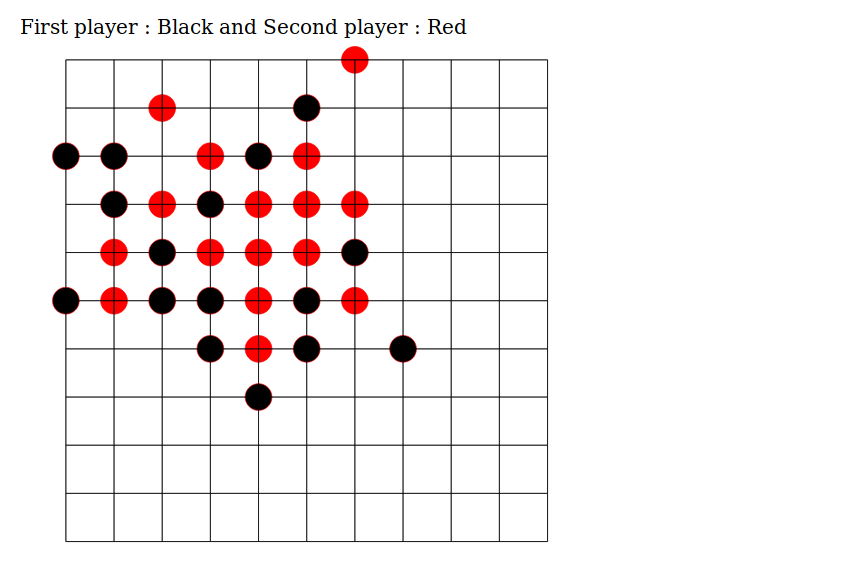
\includegraphics[width=0.90\textwidth]{display.png}
    \caption{}
    \label{fig:display}
\end{figure}
\underline{Remarque}: On a pas commité le source correspondant à cet affichage vu des raisons de simpliification, et qu'il n'était pas directement demandé par l'énoncé des sujets.
\subsection{Un serveur fonctionnant avec plusieurs joueurs}
Une autre chose à laquelle on a pensé est de créer un serveur qui marche avec plusieurs joueurs, mais vu la contrainte du temps, nous n'avons pas réussi à la faire mais notre serveur peut plus ou moins facilement être adaptable à plusieurs joueurs.

\section{Résultats finaux}
L'image ci-dessous est la représentation d'un graph. Les cercles en rouge désignent les sommets, les lignes en noir représentent les aretes reliant les sommets. cette map est obtenue à l'aide du lien :
$http://localhost:9000/$
\begin{center}
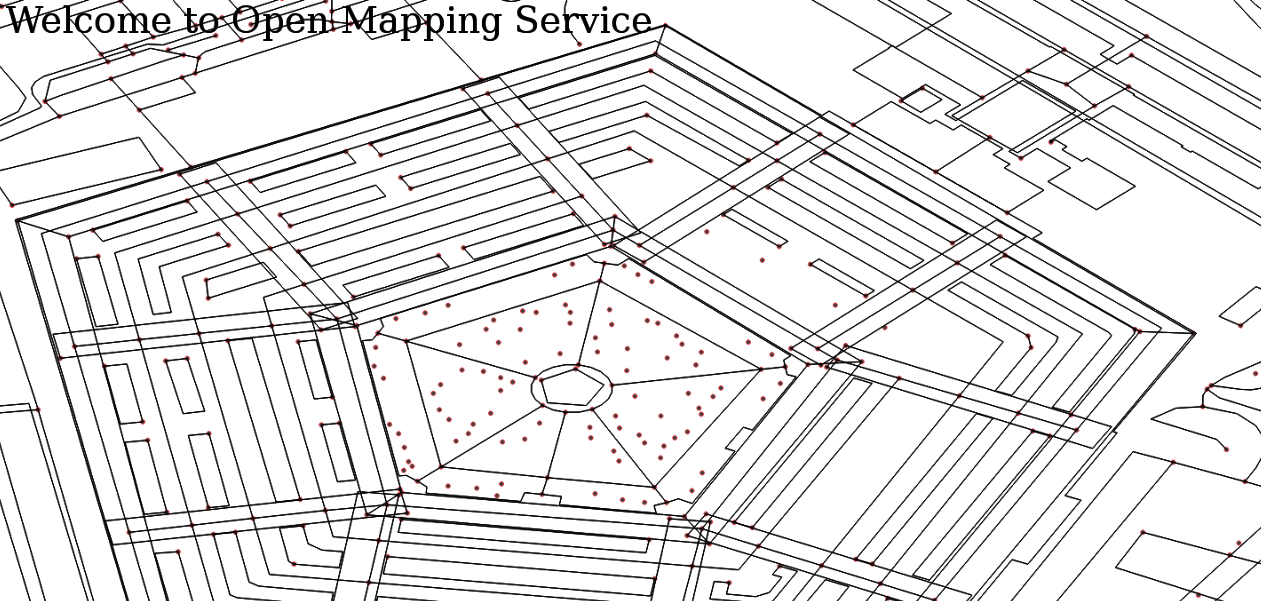
\includegraphics[scale=0.3]{map1.png}
\end{center}


Dans cette seconde image on représente les sommets et les aretes en plus du chemin reliant deux sommets. Le choix de couleurs différentes est tout à fait possible. cette map est obtenue à l'aide du lien :
$http://localhost:9000/route?start=392014874\&end=392015296$
\begin{center}
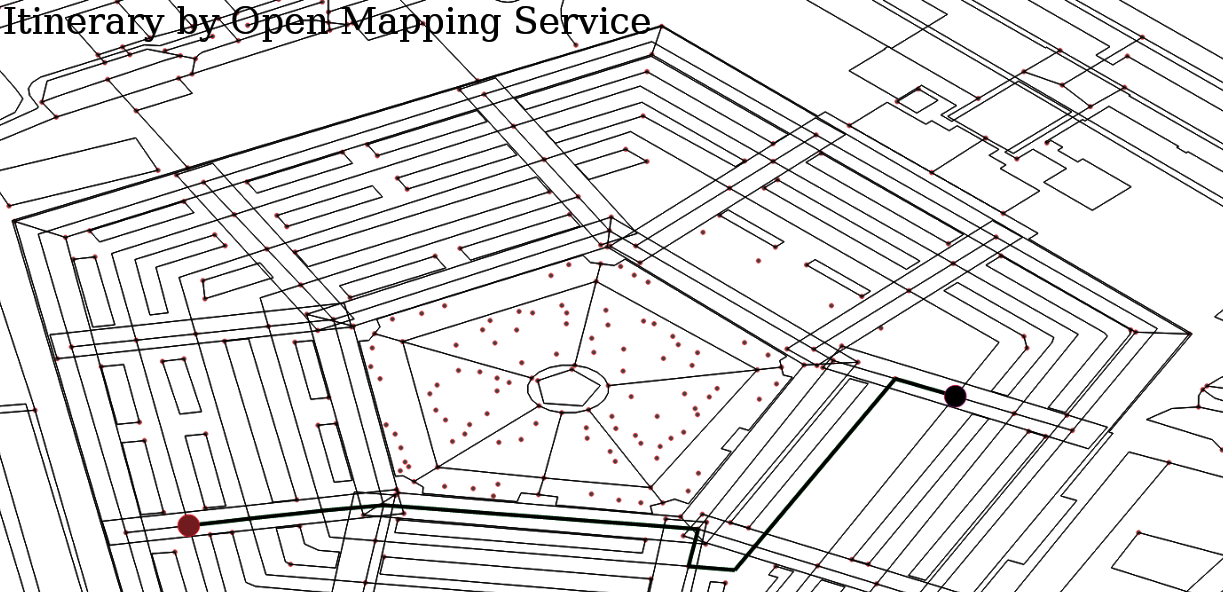
\includegraphics[scale=0.3]{route1.png}
\end{center}

\newpage
Dans cette troisième image, on représente les sommets et les arretes et le chemin le plus court reliant deux sommets choisis aléatoirement. Le cercle en bleu désigne le sommet de départ et le cercle en rouge désigne le sommet d'arrivée. Vous pouvez constater qu'au dessus de chaque \textit{sommet/cercle} figure la distance (en km) séparant ce sommet du sommet de départ. cette map est obtenue à l'aide du lien :
$http://localhost:9000/distance?start=392014874\&end=392015296$

\begin{center}
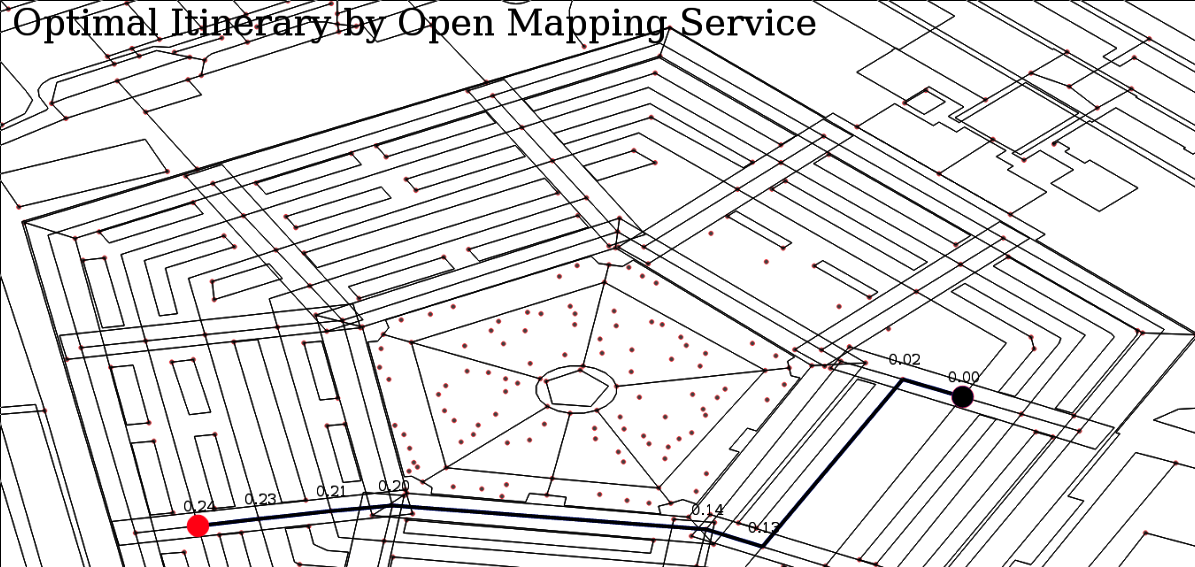
\includegraphics[scale=0.3]{distance1.png}
\end{center}
\newpage
\section{Conclusion}
Dans ce projet notre premier défi était de passer des fichiers au format osm au format graph. Ensuite, s'est posée la question de quelles structures choisir pour le graph et pour les sommets. En plus de ces contraintes techniques, il a fallu songé à comment est-ce qu'on peut pondérer notre graph d'où l'usage de \textit{la formule de haversine}, comment trouver l'itinéraire entre deux sommets d'où \textit{le parcours en profondeur} et ,enfin, comment trouver le plus court chemin entre deux sommets d'où l'implémentation de \textit{l'algorithme de dijkstra}. Une première implémentation de dijkstra a nécessité l'usage de liste des paires. L'idée de la mise à jour des distances et des prédecesseurs étant centrale dans dijkstra , il a fallu que l'on opte pour une seconde version de dijkstra qui , elle, utilise les hash-table. Une fois la manipulation des graphes finie, il a fallu que l'on travaille sur comment représenter les graphes, pour cela on a utilisé des fonctions permettant de placer des sommets, de tracer des aretes, de marquer les distances correspondant à chaque sommet mais aussi qui permettent de tracer à partir de l'algorithme de dijkstra le plus court chemin séparant deux sommets. Enfin, l'outil principal qui nous a permis de manipuler le graph est les tables de hachage. 
 \newpage
\end{document}
